
\section{UV-Mutagenese} % Nicki

\begin{mechanism}[title=Definieren Sie die Mutationstypen]
\begin{enumerate}
    \item  \textbf{Auxotroph-Mutanten} (Mangel-Mutanten) haben einen Block in einem aufbauenden (anabolischen) Stoff-
wechselweg, der die Synthese eines Zellbausteins (Aminosäure, Vitamin) verhindert. Wachstum kann nur
nach Zusatz des „Bedürfnisses“ zum Medium erfolgen.
\item \textbf{Fermentativ-Mutanten }haben einen Block in einem abbauenden (katabolischen) Stoffwechselweg, wo-
durch die Fähigkeit zur Vergärung einer bestimmten Kohlenstoffquelle (z. B. des Zuckers Lactose) verlo-
ren geht.
\item \textbf{Resistenz-Mutanten} gegen Antibiotika oder Bakteriophagen haben eine Resistenz auf Grund verschie-
dener Mechanismen, wie veränderter Permeabilität der Zellwand, Änderung in der Ribosomenstruktur,
Produktion von Enzymen, die Antibiotika abbauen.
\end{enumerate}
Bzw. auf Sequenz-Ebene (wird nicht gemeint sein...)
\begin{itemize}
    \item \underline{Deletion}: Verlust von Basen 
    \item \underline{Insertion}: Zuästzliche Basen
    \item \underline{Inversionen}: Verdrehung von Basensequenzen um 180°
    \item \underline{bewegliche genetische Elemente}: Insertionen oder unexakt herausgeschnittene Elemente 
    \item \underline{Translokation}: Verlagerung einer Basensequenz 
    \item \underline{Transition}: Eine Pyrimidin-Base wird durch eine anderen Pymiridin-Base ausgetauscht bzw. das selbe mit Purin-Basen
    \item \underline{Transversion}: Purin durch Pyrimidinbase ersetzt oder andersherum 
\end{itemize}
Purinbasen: A,G; Pyrimidinbasen: C,T
\end{mechanism}

\textbf{Auswirkungen von Mutationen:} unterschiedlich, je nach dem wo sie auftreten
\begin{itemize}
    \item in regulativen Elementen (Regulationsmutationen)
    \item in Kodiebereichen (Genmutationen)
    \item in Introns
    \item in anderen DNA-Elementen
\end{itemize}

\textbf{selektive Marker:} Wachstum dieser Mutationstypen kann mit Hilfe eines geeigneten Mediums selektiv gefördert oder unterdrückt werden\\
\textbf{nicht-selektive Marker:} Mutationen, die nicht-lebensnotwendige Funktionen betreffen\\

\textbf{Mutagene Agenzien:} UV-Strahlen (ungerichtet, relativ gleich verteilt, wenig gefährlich), chemisch verändernde Agenzien, Basenanaloge, interkaliernde Agenzien\\

\textbf{Prinzip der Selektion:} Mutante hat nicht die Fähigkeit eine gewisse Aminosäure (o.Ä.) zu produzieren. Es wird auf Minimalmedium (MM) mit Zugabe der fehlenden Aminosäure ausplattiert.Im folgenden wird auf MM (ohne Zugabe!) ausplattiert. Da die Aminosäure lebensnotwendig ist, kann die Mutante nicht auf MM wachsen und so als Mutante identifiziert werden.

\begin{mechanism}[title=Wofür codiert das lacZ-Gen?]
Für $\beta$-Galactosidase 
\end{mechanism}

\begin{mechanism}[title=Welchen Nutzen und welche Funktion hat das lacZ-Gen in der Genomik?]
\begin{itemize}
    \item Reportergen in Klonierungsvektoren (Blau-Weiß-Screening)
    \item wird häufig in Klonierungsvektoren integriert, um die erfolgreiche Integration von DNA-Fragmenten zu überprüfen
\end{itemize}
\end{mechanism}

\begin{mechanism}[title=Wofür ist das Produkt des lacZ-Gens verantwortlich? ]
$\beta$-Galactosidase hat zentrale Rolle im Laktosestoffwechsel von Bakterien: 
Hydrolyse von Laktose in Glukose und Galaktose oder Isomerisierung in Allolactose; Regulation des lac-Operons über Allolactose (Induktor)
\end{mechanism}

\begin{mechanism}[title=Wofür wird das lacZ in der Gentechnik verwendet?]
Reportergen und als Werkzeug zur Selektion und Identifizierung von rekombinanten Klonen verwendet.
\end{mechanism}

\subsection{Wildtyp Funktionsweise}
Lactose wird nur verwertet, wenn keine Glucose verfügbar ist. Dann wird Lactose in Glucose und Galactose gespalten

Irgendwo muss noch was hin zu "LacZ Mutationsraten Bestimmung" (aus einer Gedächtnisprotokoll) und Mutationsrate von lacZ


\begin{mechanism}[title=Beschriften]
\begin{figure}[H]
    \centering
    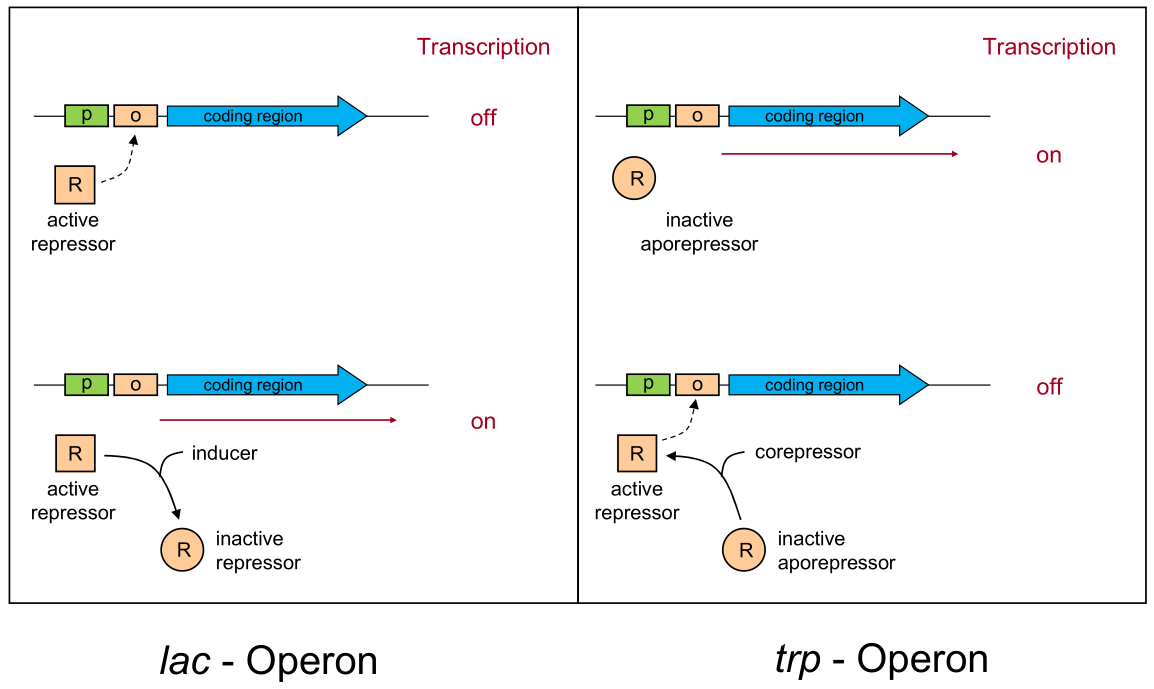
\includegraphics[width=12cm]{images/repressorbildfilled.png}
\end{figure}
\end{mechanism}

% Liliana
%% 

\section{Tn5-Mutagenese} 
Man inaktiviert Gene durch Mutagenese\index{Mutagenese}, um herauszufinden welche Funktion sie haben. Ein sehr verbreitetes und effizientes Mutagenese\index{Mutagenese}-System ist die Mutagenisierung durch das Transposon\index{Transposon} Tn5.
\index{Mutagenese} \index{Transposon!Tn5}

\subsection{Transposons}
\begin{mechanism}[title=Definition Transposon]
Mobile genetische Elemente und können sich von einem Ort im Genom zu einem anderen bewegen, entweder durch einen "Kopieren-und-Einfügen"-Mechanismus oder durch einen  "Ausschneiden-und-Einfügen"-Mechanismus.
\end{mechanism}

\subsubsection{Klassen von Transposons}
\begin{itemize}
    \item Klasse I: Zentraler Bereich ist von zwei \glspl{iselement}\index{IS-Element}n flankiert
    \item Klasse II: Zentraler Bereich trägt die \gls{transposase} und ist von kurzen „inverted repeats“ flankiert 
\end{itemize}\index{Transposon!Klassen von}

\begin{mechanism}[title=Zu welcher Transposon-Klasse gehört Tn5?]
Das gehört zu Klasse I. \\ \newline
Zwei IS50 flankieren Resistenzgene und eine Tn5 Transposition wird über die  IS50R-Transposase\index{Transposase!IS50R} vermittelt.
\end{mechanism} 

\subsubsection*{IS-Elemente} \label{l:is-element}
\glspl{iselement}\index{IS-Element} sind Insertionssequenzen und die einfachsten "springenden Gene" mit einer Länge unter 2 kb. Sie tragen konservierte \glspl{ir} an den Enden und kodieren \gls{transposase}-Enzyme, welche den Sprung (Transposition) vermitteln. \glspl{ir} fungieren als Erkennungssequenzen für die \gls{transposase}. \\
Der Insertionsort ist im Prinzip sequenzunabhängig, aber es gibt Hotspots, an denen ofter eingefügt wird. \\
Bei der Integration werden \glspl{dr} erzeugt ("Fußabdrücke"). \\
\glspl{iselement}\index{IS-Element} sind an autonome \glspl{replikon} gebunden (Chromosom, Plasmid, Bakteriophage) und die Kopienzahl von \glspl{iselement}\index{IS-Element}n im Genom ist stammspezifisch.

 
\begin{mechanism}[title=Welche der folgenden Eigenschaften hat ein IS-Element]

\begin{itemize} 
    \item[[ ]] suicide
    \item[[X]] \gls{ir}
    \item[[ ]] \gls{replikase}
    \item[[X]] \gls{transposase}
    \item[[?]] broad host range
    \item[[X]] repeats
\end{itemize}
\end{mechanism}

\begin{mechanism}[title=Zeichne ein IS-Element]
\begin{figure}[H]
    \centering
    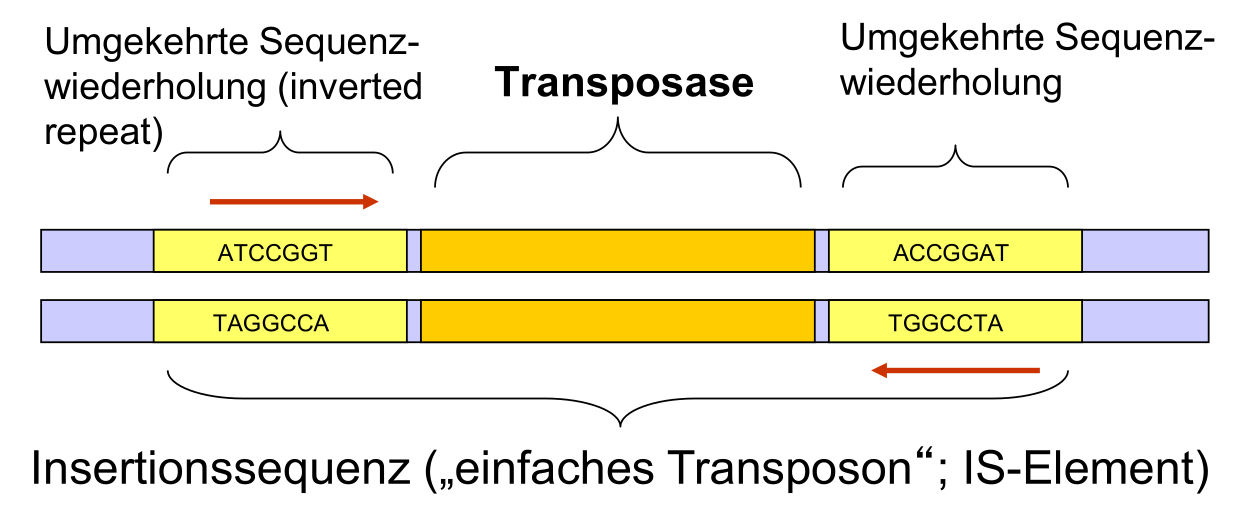
\includegraphics[width=12cm]{images/iselement.png}
\end{figure} \index{IS-Element}
\end{mechanism}


\subsubsection{Transpositionsmechanismen} \index{Transpositionsmechanismen}
\begin{itemize}
    \item \textbf{Konservative Transposition}: "cut and past"
    \item \textbf{Replikative Transposition}: "copy and paste" 
\end{itemize}
\index{Transposition!konservative}\index{Transposition!replikative}
\begin{mechanism}[title=Was ist der Tanspositionsmechanismus von Tn5?]
\todo
\begin{itemize}
    \item[[ ]] konservativ
    \item[[ ]] multiplikativ
    \item[[ ]] transpositiv
    \item[[ ]] replikativ
\end{itemize}
\end{mechanism}

\subsubsection{Tn5}
Tn5 bietet die Möglichkeit der \textbf{positiven Selektion}, also dass man die Bakterien selektiert, bei denen die Mutagenese\index{Mutagenese} funktioniert hat. Das geht, weil Tn5 eine Antibiotikumresistenz gegen Neomycin/Kanamycin beinhaltet und diese bei erfolgreicher Mutagenese\index{Mutagenese} auf die Bakterien über geht. Man sagt auch es wird auf positive Transpositionsereignisse selektiert. \\ \newline
Damit Tn5 erfolgreich vermittelet werden kann, braucht das vermittelnde Bakterium (der Donor) \glspl{transferfunktion} (eine tra-Region) auf seinem Chromosom und das zu vermittelnde Plasmid mit Tn5 braucht eine \gls{mob} und natürlich die Antibiotikumresistenz.  Die Tn5-vermittelte Antibiotikumresistenz bleibt im Rezipientenstamm nur dann erhalten, wenn das Transposon\index{Transposon} vom Plasmid auf die chromosomale DNA transferiert wurde, die Mutagenese\index{Mutagenese} also erfolgreich war. \\ \newline
Die resultierenden \glspl{transkonjugant} können dann auf Mutationen untersucht werden, das heißt man untersucht welche Funktionen (bspw. Stoffwechselwege) gestört sind. 

\begin{mechanism}[title=Zeichnen Sie das tn5 Transposon detailliert]
\begin{figure}[H]
    \centering
    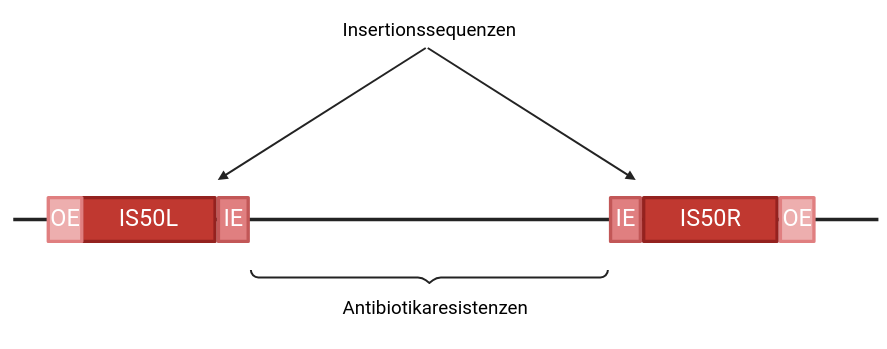
\includegraphics[width=12cm]{images/tn5.png}
\end{figure}
\begin{figure}[H]
    \centering
    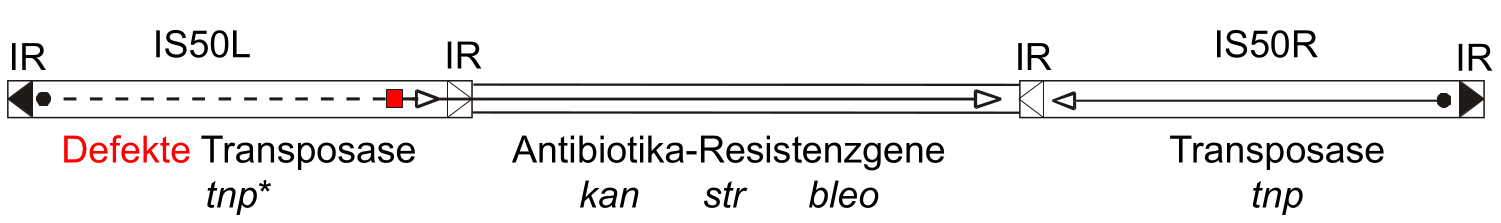
\includegraphics[width=12cm]{images2/tn5skript.png}
\end{figure}
\end{mechanism}

\begin{mybox}[title=Was sind Transkonjuganten?]
\glspl{transkonjugant} sind die bei einer Konjugation neu entstandenen F+-Zellen. 
\end{mybox}

Es gibt bestimmte "Mobilisierungsstämme" von Bakterien, die als Donoren dienen sollen. 

%\subsubsection{Tn3}

\subsection{Ablauf des Experiments}

\subsubsection{Kreuzung von Donor- und Rezipientenstamm}
\begin{enumerate}
    \item Der mit dem zu mobilisierenden Plasmid versehene Donor wird in \gls{lbmedium} selektiv angezogen. 
    \item Der Rezipient wird über Nacht in\gls{tymedium} selektiv angezogen.
    \item logarithmisch wachsenden Donorkultur wird mit stationärer Rezipientenkultur im Eppendorfgefäß gemischt und anschließend abzentrifugiert
    \item Überstand abgießen und Zellen vorsichtig im Rücklauf resuspendieren
    \item \gls{Nitrocellulose-Filter} werden auf werden auf \gls{typlatte} (unselektiv) steril aufgelegt und die Platten vorgewärmt
    \item die Kreuzungssuspension wird auf die Nitrocellulose-Filter pipettiert und die Platten mindestens über Nacht inkubiert
    \item Die Filter werden steril in ein Eppendorfgefäß mit sterilem Wasser überführt und abgeschwemmt (stark vortexen), dann bei RT inkubiert
    \item Transkonjuganten-Zellsuspension und eine $10^{-1}$ Verdünnung werden auf \gls{typlatte} selektiv ausplattiert und für ca. 3 Tage inkubiert.
\end{enumerate}
\subsubsection{Verdünnungsreihen und Titerung}
\begin{enumerate}
    \item von den verwendeten Donor- und Rezipientenkulturen werden Verdünnungsstufen erstellt
    \item von allen Verdünnungsstufen wird etwas auf \gls{lbmedium} oder \gls{tymedium} gleichmäßig verteilt (ausgespatelt, ausplattiert) - diese Platten dienen der Titerung der verwendeten Bakterien
\end{enumerate}
\begin{mybox}[title=Was ist Titierung?]
Ersteinmal heißt es \gls{titerung}.  Der \gls{titer} ist ein Maß für die Menge der Bakterien und die \gls{titierung} ist das Verfahren zur Bestimmung der Konzentration der Bakterien (in einer wässrigen Lösung). 
\end{mybox} 
% evtl mehr todo? Klären in welchen Einheiten das ist oder so? 



\begin{mechanism}[title=Definition Lebendtiter]
Die Konzentration lebender Mikroorganismen, wie Bakterien, Viren oder Hefen, in einer bestimmten Volumeneinheit einer Flüssigkeit. Der Lebendtiter wird normalerweise in koloniebildenden Einheiten pro Milliliter (KBE/ml) oder Plaque-bildenden Einheiten pro Milliliter (PFU/ml) ausgedrückt, abhängig von der Art der Mikroorganismen und der verwendeten Nachweismethode. 
\end{mechanism}
 
 
  
 
\begin{mechanism}[title=Wie bestimmt man einen Lebendtiter? ausführlich]
\begin{itemize}
    \item Homogenisieren der Probe, um eine gleichmäßige Verteilung der Mikroorganismen zu gewährleisten
    \item Serielle Verdünnungen
    \item Plattieren der Verdünnungen auf Petrischalen mit Nährmedium
    \item Inkubieren der Platten
    \item Koloniezählung
    \item Berechnung des Lebendtiters: \\ 
    \textit{Lebendtiter (KBE/ml) = }$\frac{\# Kolonien}{Volumen \ der \ Plattierung (ml)} \times$ \textit{Verdünnungsfaktor}
\end{itemize}
\end{mechanism}





\begin{mybox}[title=Warum macht man Verdünnungsreihen?]
Die Bakterien lassen sich in höheren Verdünnungsstufen leichter zählen, das Ergebnis kann anschließend wieder auf ursprüngliche Konzentration zurückgerechnet werden. \\
Also damit man die Bakterien zählen kann. 
\end{mybox}

\subsubsection{Identifizierung und Charakterisierung von Tn5-Mutanten} 
Transkonjuganten auf verschiedene Medien stochern, je nach Medium sollten nur bestimmte Mutanten wachsen.



\begin{mechanism}[title=Welche Eigenschaften muss ein Vektor für tn5 Mutagenese auf jeden Fall aufweisen?]
\begin{itemize}
    \item  die Tn5-Transposon-Sequenz enthalten, einschließlich der invertierten Wiederholungen,
    \item ein Selektionsmarker (meistens Antibiotikaresistenzgen)
    \item Transposase-Gen
    \item Replikationsursprung
    %check \todo 
\end{itemize}
\end{mechanism}



\begin{mechanism}[title=Was ist ein SuicidePlasmid und wofür wird es verwendet?]
Suicide-Plasmide sind Plasmide, welche in einem bestimmten Wirtsbakterium nicht repliziert werden können.
Sie werden eingesetzt für gezielte Mutationen bei Bakterien. \index{Suicide-Plasmid}  
\end{mechanism}

\begin{mechanism}[title=Welche der folgenden Eigenschaften hat ein suicide-Vektor]
\todo 
\begin{itemize}
    \item[[ ]] Transposon\index{Transposon}
    \item[[ ]] Breiter Wirtsbereich
    \item[[ ]] IS-Element
    \item[[ ]] Eingeschr¨ankter Wirtsbereich
    \item[[ ]] Mutator
    \item[[ ]] oriT
\end{itemize}
\end{mechanism}

\todo: "Tn5 Mutagenese Antibiotika Strept. Kana. Donor Rezipient (ca 6 S¨atze zum ankreuzen)" aus Gedächtnisprotokoll

+ \todo: "estriktionsschnittstelle (Bakteriophage Lambda) KpnI, Sequenzierung nicht m¨ogl., EcoRI
und HindIII bekannt" auch aus Gedächtnisprotokoll


%%%%%%%%%%%%%%%%%%%%%%%%%%%%%%%%%%%%%%%%%%%%%%%%%%%%%%%%%%%%%%%%%%%%%%%%%%%%%


% Liliana
\section{Restriktionskartierung} \label{sec:Restriktionskartierung} \index{Restriktionskartierung}
Eine Restriktionskarte zeigt Positionen der Schnittstellen einzelner Restriktionsenzyme auf der DNA eines bestimmten Genoms oder Plasmids. Dadurch kann man anhand der Schnittstellen von unbekannten Fragmenten diese Fragmente identifizieren. 
Siehe auch \nameref{sec:Restriktionsendonuklease} auf \pageref{sec:Restriktionsendonuklease}
\subsection{Klassen von Restriktionsenzyme}
\begin{table}
\begin{adjustbox}{angle=90}
    \centering
    \begin{tabular}{p{0.5cm} p{4cm} p{3cm}p{3cm}p{2cm}p{3cm}p{3cm}}
        \textbf{Typ} & \textbf{Wirkung} & \textbf{Spaltungsort} & \textbf{transferieren}... & \textbf{Kofaktoren} & \textbf{Zusammenhang Methylierung} & \textbf{Sonstiges} \\ \\
        I. & funktionieren als \glspl{pentamereenzymkomplexe} & zufällig, $>$ 1000 bp von Erkennungssequenz & Methylgruppe von \gls{sam} & \gls{sam}, \gls{atp}, $Mg^{2+}$  & durch Meth. gehemmt \\
        II. & zwei separate Enzyme arbeiten unabhängig voneinander &  & & & durch Meth. gehemmt   \\
        III. & wirkt als Heterooligomer für Erkennung und Methylierung & 25-30 bp downstream Methylgruppe von \gls{sam} & \gls{sam}, \gls{atp}, ${Mg}^{2+}$ & durch Meth. gehemmt \\
        IV. &  &  & & & erkennt und schneidet nur methylierte DNA.\\
        V. &  verwenden sog. \gls{grna} um spezifische Sequenzen zu erkennen und zu schneiden 
    \end{tabular}
\end{adjustbox}
    \caption{Klassen von Restriktionsenzyme}
    \label{tab:klassenrestriktionsenzyme}
\end{table}
\todo klassen und deren Eigenschaften
\begin{mechanism}[title=Was sind die Eigenschaften von Restriktionsenzyme der Klasse II?]
\todo
\end{mechanism}

\begin{mechanism}[title=Beschreiben Sie die Eigenschaften von Restriktionsendonuklease II]
\begin{itemize}
    \item binden an spezifische DNA-Sequenzen (spezifische Erkennungssequenzen)
    \item schneiden die DNA innerhalb oder in unmittelbarer Nähe der Erkennungssequenz (Präziser und reproduzierbarer Schnitt)
    \item kann \gls{blunt ends} und \gls{sticky ends} erzeugen 
    \item Mg2+-Ionen als Cofaktor, aber keine ATP- oder S-Adenosylmethionin-Cofaktoren (Katalytische Unabhängigkeit)
\end{itemize}
\end{mechanism} 

\subsection{Der Bakteriophage Lambda}
\todo
\begin{mechanism}[title=Wie schützen sich Bakterien vor fremder DNA?]
Durch \glspl{restriktionsendonuklease}. \glspl{restriktionsendonuklease} sind Enzyme, die DNA an bestimmten Positionen schneiden können. Sie erkennen fremde DNA (meist) am fehlenden Methylierungsmuster und zerschneiden dann Fremd-DNA. Sie treten im Bakterium immer zusammen mit DNA-\glspl{methyltransferase} auf, die der bakterieneigenen DNA kennzeichnende Muster aufprägen. Die Kombination aus einer \gls{restriktionsendonuklease} und einer \gls{methyltransferase} nennt man \gls{rmsystem}.
\end{mechanism}
\subsection{Ablauf der Kartierung}
\todo
\subsubsection{Spaltung von $\lambda$-DNA mit Restriktionsenzymen}
\todo
\subsubsection{Agarose-Gelelektrophorese der Spaltung}
\todo
\subsubsection{Kartierung des $\lambda$-Genoms}
\todo



\begin{mechanism}[title=Wie kann man eine Restriktionsschnittstelle kartieren ohne Sequenzierung und mit Hilfe anderer Restriktions Fragmentlängen?]
\todo
\end{mechanism}

\section{Techniken der in vitro Gentechnologie}
\todo
\subsection{Ablauf des Experiments}
\todo
\subsubsection{Isolierung von Plasmid-DNA für DNA-Klonierung}
\todo
\subsubsection{Agarose-Gelelektrophorese}
\todo

\section{Sequenzierung von Plasmid-DNA}
\todo

\section{Expression von Proteinen}
\todo

\subsection{Ablauf des Experiments}
\todo
\subsubsection{Überexpression des GFP-Proteins in E. coli}
\todo
\subsubsection{Polyacrylamid Gelelektrophorese} \index{SDS-Page}
\todo
\subsubsection{Färbung von Proteingelen}
\todo

\section{Genetischer Fingerabdruck}
\todo

\begin{mechanism}[title=Definition Genetischer Fingerabdruck]
\todo
\end{mechanism}

\subsection{Ablauf des Experiments}
\begin{mechanism}[title=Wie ist der Ablauf zur Gewinnung eines genetischen Fingerabdrucks?]
\todo
\end{mechanism}
\begin{mechanism}[title=Chromosomale DNA-Extraktion - allgemeiner Ablauf]
\begin{itemize}
    \item Probe gewinnen 
    \item Zelllyse
    \item Proteinabbau
    \item Zentrifugation: Entfernung von Zelltrümmern
    \item DNA-Reinigung
    \item DNA-Fällung
    \item Waschen der DNA
\end{itemize}
\end{mechanism}
\subsubsection{DNA-Isolation aus Zellen der Mundschleimhaut}
\todo

\subsubsection{PCR-Amplifikation}
\todo

\subsubsection{Agarose-Gelelektrophorese der PCR Proben}
\todo

\subsubsection{Auswertung}
\todo

 
